Este capítulo presenta la validación del sistema Voctomix~2.0 a lo largo de los cuatro
escenarios de despliegue sobre los que se ha desarrollado y probado el proyecto.
Para cada escenario se describe el entorno utilizado, los objetivos de validación y
los resultados obtenidos. Se incluyen además pruebas de rendimiento que caracterizan
el comportamiento del sistema bajo carga real.

\section{Escenarios de despliegue evaluados}
\label{sec:escenarios}

La validación del sistema se ha llevado a cabo de forma progresiva a través de cuatro
escenarios que cubren desde el entorno de desarrollo inicial hasta el despliegue
orquestado en Kubernetes. Cada escenario añade una garantía de calidad que el anterior
no podía ofrecer. La tabla~\ref{tab:escenarios} resume sus características principales.

\begin{table}[H]
  \centering
  \caption{Comparativa de los cuatro escenarios de despliegue evaluados.}
  \label{tab:escenarios}
  \begin{tabular}{|l|c|c|l|}
    \hline
    \textbf{Escenario} & \textbf{Máquinas} & \textbf{Orquestación} & \textbf{Objetivo de validación} \\
    \hline
    1 PC (desarrollo)   & 1 & Manual / scripts    & Funcionalidad del pipeline \\
    2 PCs en LAN        & 2 & Manual / scripts    & Comunicación en red real \\
    Docker Compose      & 1 & Docker Compose      & Reproducibilidad y portabilidad \\
    Kubernetes          & 1 & Kubernetes/Minikube & Orquestación y resiliencia \\
    CyberNEMO Trial~3   & Clúster UPM & Kubernetes (producción) & Integración en proyecto real \\
    \hline
  \end{tabular}
\end{table}

\subsection{Escenario 1: un PC (entorno de desarrollo)}

Durante las primeras semanas de desarrollo todo el sistema se ejecutó en un único
equipo: voctocore, las cuatro fuentes FFmpeg, el stream blanker, el servicio de
telemetría y voctogui corrían simultáneamente en la misma máquina. Este escenario
permitió iterar rápidamente sobre el código sin necesidad de sincronizar dos equipos
ni gestionar direcciones IP. Fue el entorno en el que se implementaron y depuraron
la totalidad de los componentes: composites, overlays, rotulación dinámica, scripts
de arranque y el servicio de telemetría.

\subsection{Escenario 2: dos PCs en red local}

Una vez que el sistema era funcional en un único equipo, se validó su comportamiento
en red: voctocore y las fuentes FFmpeg se ejecutaron en el PC servidor mientras que
voctogui se conectó desde un segundo equipo mediante una red local. El objetivo de
este escenario no era añadir nuevas funcionalidades sino confirmar que la arquitectura
cliente-servidor funcionaba correctamente en un entorno distribuido real: que los
cortes de cámara eran efectivos sin retardo apreciable, que las previsualizaciones
JPEG llegaban fluidas al realizador y que el servicio de telemetría recibía los estados
de la GUI del PC remoto mediante HTTP POST. Se verificó además la latencia de
conmutación bajo condiciones de red WiFi y cableada.

\subsection{Escenario 3: Docker Compose}

El tercer escenario eliminó la necesidad de instalar manualmente GStreamer, Python y
sus dependencias en el equipo anfitrión. Con la imagen Docker construida a partir del
\texttt{Dockerfile} descrito en la sección~\ref{sec:docker}, el sistema completo se
despliega con un único comando:

\begin{verbatim}
docker compose up
\end{verbatim}

Docker Compose gestiona el orden de arranque mediante \textit{healthchecks}, levanta
los diez servicios definidos en \texttt{docker-compose.yml} y expone los puertos
necesarios al sistema anfitrión. La GUI se conecta desde el \textit{host} exactamente
igual que en el escenario de dos PCs, utilizando \texttt{localhost} como destino.

\subsection{Escenario 4: Kubernetes con Minikube}

El escenario más avanzado migra la orquestación de Docker Compose a Kubernetes
ejecutándose localmente sobre Minikube. Los manifiestos YAML definen el ciclo de vida
declarativo de cada servicio, con \textit{readiness probes} que garantizan el orden
correcto de arranque sin depender de \texttt{sleep} ni lógica de espera en los scripts.
El script \texttt{launch\_k8s.sh} comprueba si el clúster ya está activo antes de
inicializarlo, establece el \textit{port-forward} necesario para que voctogui acceda
a los puertos del pod y muestra los logs de telemetría en tiempo real. Este escenario
valida que el sistema puede operar sobre infraestructura de orquestación estándar de
la industria.

\subsection{Escenario 5: integración en el proyecto CyberNEMO (producción real)}
\label{sec:escenario_cybernemo}

Además de los cuatro escenarios de laboratorio anteriores, Voctomix~2.0 fue desplegado
en el entorno de producción real del proyecto europeo de investigación \textbf{CyberNEMO},
liderado por la UPM. En este contexto, el sistema actuó como motor de producción
audiovisual conectado al clúster Kubernetes de la universidad e integrado con los
componentes de ciberseguridad Zero Trust del proyecto, que protegen el acceso y la
integridad del contenido multimedia durante la producción en directo.

El servicio de telemetría con RabbitMQ publicó los eventos del mezclador en tiempo real
en colas consumidas por los sistemas de monitorización del proyecto, lo que permitió
verificar el correcto funcionamiento de la cadena de producción completa en un entorno
de red real. Este escenario validó la capacidad del sistema para integrarse en una
infraestructura de investigación activa sin necesidad de modificar el núcleo de la
aplicación.

\begin{figure}[H]
  \centering
  \begin{subfigure}[t]{0.54\textwidth}
    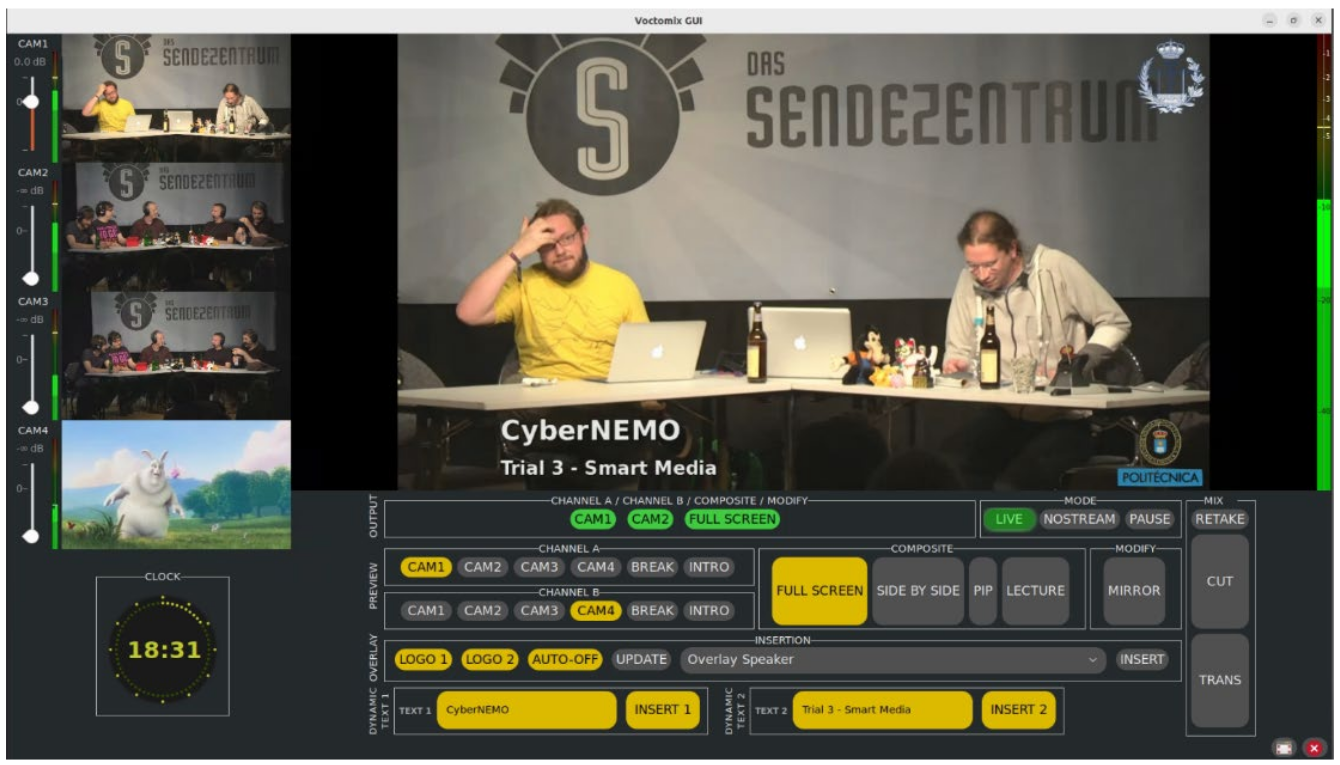
\includegraphics[width=\textwidth]{figuras/voctogui_cybernemo1.png}
    \caption{Interfaz del operador (voctogui).}
    \label{fig:voctogui_cybernemo_gui}
  \end{subfigure}
  \hfill
  \begin{subfigure}[t]{0.42\textwidth}
    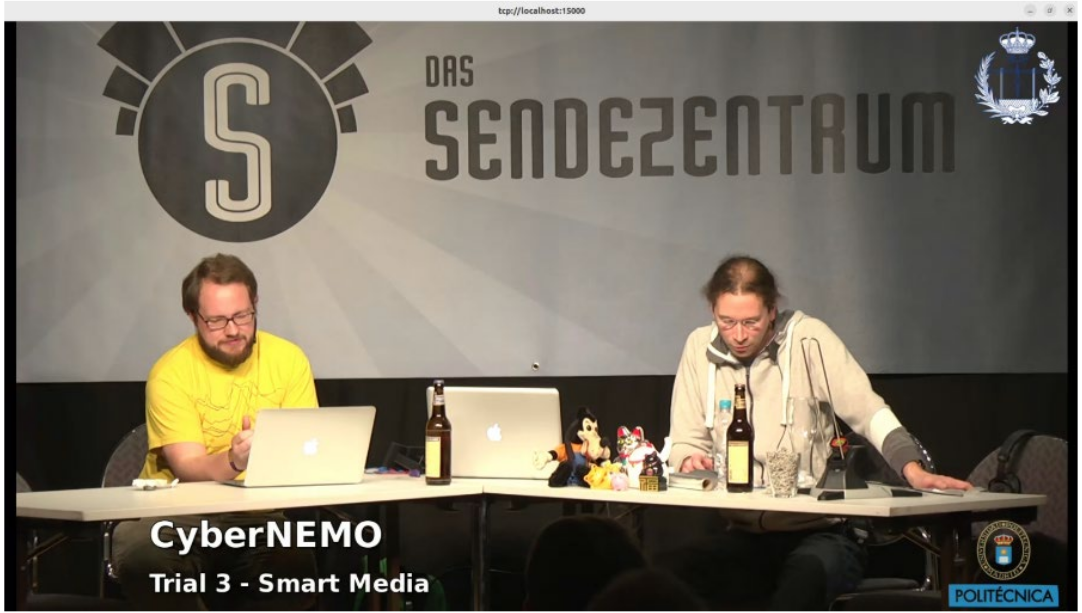
\includegraphics[width=\textwidth]{figuras/voctogui_cybernemo2.png}
    \caption{Señal de programa vista por el espectador.}
    \label{fig:voctogui_cybernemo_out}
  \end{subfigure}
  \caption{Voctomix~2.0 en producción real durante la integración con CyberNEMO (UPM).}
  \label{fig:voctogui_cybernemo}
\end{figure}
